\documentclass[12pt]{article}
\usepackage{graphicx,float}
\usepackage{listings}
\usepackage{xcolor}
\usepackage[left=3cm,right=3cm]{geometry}
\graphicspath{ {./fig/} }

\title{CS419(M): Programming Assignment-1}
\author{Prateek Garg, 20D070060}
\date{31st March 2022}
\begin{document}
\noindent
\maketitle
\section{Preleminary Questions}
\begin{itemize}
    \item Since we are predicting a single quantity, the quality of wine based on given data,
    this must treated as a regression problem only with some modified output values. 
    CLassification deals with categorizing data points into seperate classes which is not the case here
    \item Another metric can be \textbf{Mean Absolute error}, $$\frac{\sum_{i=1}^{n} |y_i-H(x_i)|}{n}$$ 
    This can be interpreted as average of distances from the true value of quality.
\end{itemize}

\section{Gradient Descent}
\begin{itemize}
    \item Root Mean Squared error on dev test: 0.1207951
    \item Absolute difference between the following two calls,
    \texttt{compute\_RMSE(phi,w1, y)} and \texttt{compute\_RMSE(phi, w2, y)}:1.15264436e-05
    \item We used \texttt{grad\_norm\_threshold=0.0001} which is upper limit of gradient of loss with respect to \textbf{w}.
     As soon as gradient goes below this value we stop the process
    \item Absolute difference between the following two calls, 
    \texttt{compute\_RMSE(phi,w2, y)} and \texttt{compute\_RMSE(phi, w3, y)}:1.8945e-04
    with learning rate=0.005 and number of iterations=50000
\end{itemize}

\section{Gradient Descent with p-norm regularization}
\begin{itemize}
    \item Root Mean Squared error on dev test with \textbf{p=2}: 0.12809152
    \item Root Mean Squared error on dev test with \textbf{p=4}: 0.12197416
\end{itemize}

\section{Training Data size vs RMSE}
    \begin{center}
        \makebox[0.8\textwidth]{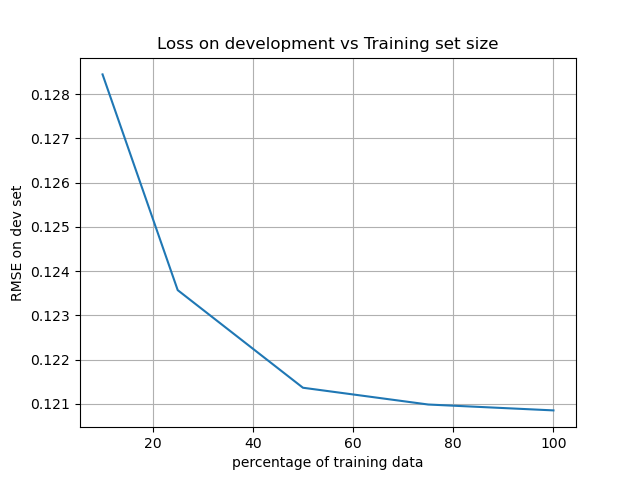
\includegraphics[width=0.8\paperwidth]{plot.png}}
    \end{center}
\section{Features}
From closed form solution, we get\\
\texttt{w*=[0.0758 0.1375 -0.3049 0.0416 0.3566 -0.0410}\\
\texttt{ 0.1659 -0.0662 -0.4573 0.1109 0.1342 0.2480]}\\
with \texttt{b*= 0.4079}\\
Since the features are normalised  the weights given by linear regression directly corresponds to the effect of a particular feature on the value.
\begin{itemize}
    \item The two most useful features thus are:  \texttt{pH, acidity}
    \item The two least useful features thus are:  \texttt{citric acid, chlorides}
\end{itemize}

\section{Regression using open-source library implementations}   
\begin{itemize}
    \item We have used \texttt{SGDRegressor} from SK-learn library.
    \item Root Mean Squared error on dev test: 0.122121
\end{itemize}
\end{document}
